% Drawing 154/05-13 -- folder 154, batch 05, archive page 88 (PDF page 89).
% Transcription: la page ne porte qu'un croquis, sans aucune légende : au crayon, un ovale et plusieurs courbes qui se croisent ; en vert, deux courbes issues d'un même point, fléchées de petites marques
% Kind: unlabelled sketch: pencil curves and two green curves. Method 2 (schematic redraw from the facsimile). Status: partial.
% Notes: Pencil, faint: an oval, a long arc on its left, a second arc rising to the right, a straight stroke crossing it and a long flat stroke. Green: one stroke that splits into two curves rising to the upper right, the upper one carrying two small arrow marks and the lower one one. The pencil curves are followed approximately; nothing is written on the page. Redrawn 2026-11-12 (issue 128): to check again.
% Coordinates: 1 unit = 1 mm = 1/100 of the crop width (bbox in page fractions: [0.16, 0.07, 0.71, 0.3]).
% Redrawn by Claude (claude-fable-5-2), issue #128, 2026-11-12; not checked by a human; not compiled (no TeX in the session).
% Rights: reproduces part of the work -- behind RENDER_TRANSCRIPTS, never published by itself.
\documentclass[tikz,border=3pt]{standalone}
\usepackage{amsmath,amssymb}
\usetikzlibrary{patterns,arrows.meta}
\tikzset{Ye/.style={yellow!80!orange}, Lg/.style={green!60!black!70}, Dg/.style={green!45!black}, pencil/.style={black!45}, struck/.style={black!35}, mpt/.style={circle,draw,inner sep=1.3pt}, pt/.style={circle,fill,inner sep=0.9pt}, opt/.style={circle,draw,fill=white,inner sep=1.1pt}}
\begin{document}
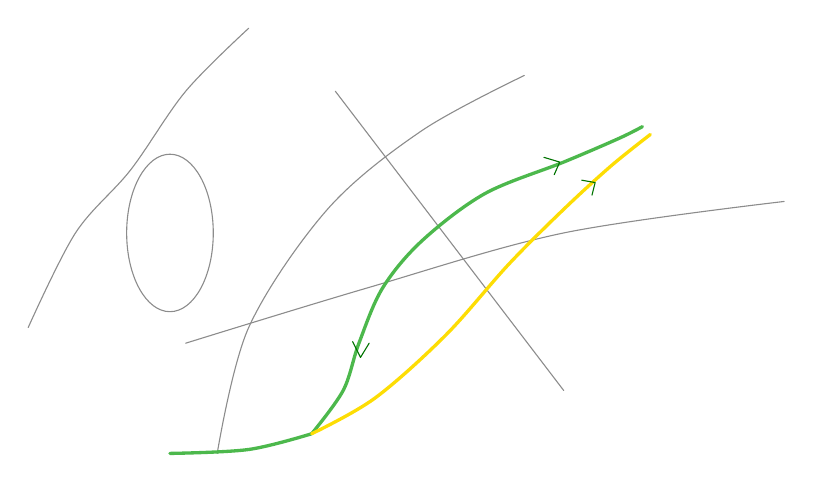
\begin{tikzpicture}[x=1mm,y=1mm,line cap=round,line join=round,font=\scriptsize]
\draw[pencil] (20,-28) ellipse[x radius=5.5, y radius=10];
\draw[pencil] plot[smooth, tension=0.55] coordinates {(2,-40) (8,-28) (15,-20) (22,-10) (30,-2)};
\draw[pencil] plot[smooth, tension=0.55] coordinates {(26,-56) (30,-40) (40,-25) (52,-15) (65,-8)};
\draw[pencil] (41,-10) -- (70,-48);
\draw[pencil] plot[smooth, tension=0.55] coordinates {(22,-42) (45,-35) (70,-28) (98,-24)};
\draw[Lg,very thick] plot[smooth, tension=0.55] coordinates {(20,-56) (30,-55.5) (38,-53.5)};
\draw[Lg,very thick] plot[smooth, tension=0.55] coordinates {(38,-53.5) (42,-48) (44,-42) (47,-35) (52,-29) (60,-23) (70,-19) (77,-16) (80,-14.5)};
\draw[Ye,very thick] plot[smooth, tension=0.55] coordinates {(38,-53.5) (46,-49) (55,-41) (63,-32) (70,-25) (76,-19.5) (81,-15.5)};
\draw[Dg] (43.2,-41.8) -- (44.2,-43.8) -- (45.3,-42);
\draw[Dg] (67.5,-18.4) -- (69.5,-19) -- (68.8,-20.6);
\draw[Dg] (72.3,-21.3) -- (74,-21.6) -- (73.6,-23.2);
\end{tikzpicture}
\end{document}
